\begin{frame}[fragile]{}
    \begin{block}{}
        \begin{itemize}
            \item We saw debuggable functions $Debuggable \: a = (a, string)$
            \item We saw multivalued functions $Multivalued \: a = [a]$
            \item Make $Debuggable$ or $Multivalued$ abstract and call it $m$
            \item In both cases you get a function $a \rightarrow m \: a$
            \item For that specific m we define $bind$ and $unit$ (the others are in function of these two)
        \end{itemize}
    \end{block}
\end{frame}

\begin{frame}[fragile]{Formal definition}
    \begin{block}{}
        A monad is a triplet $(m, bind, unit)$. $bind$ and $unit$ must satisfy a bunch of mathematical laws
    \end{block}
\end{frame}

\begin{frame}[fragile]{Informal definition}
    \begin{block}{}
        \begin{itemize}
            \item A monad is a box
            \item You define how you put a new item in this box ($unit$)
            \item You define how you can open a box to apply a function to the element inside of it ($bind$)
            \item If those two methods follow some basic rules (commutativity, ...) you can chain them nicely
        \end{itemize}
        \begin{center}
            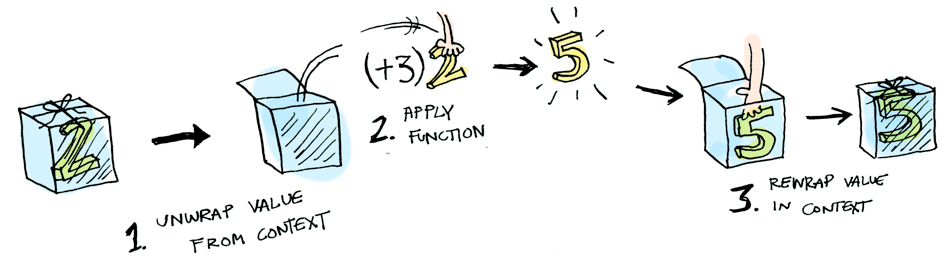
\includegraphics[scale=0.3]{images/monad_box}
        \end{center}
    \end{block}
\end{frame}

\begin{frame}[fragile]{}
    \begin{block}{What are they used for}
        The monad ('box') abstracts away a lot of computations that would be boiler plate.
        In our example passing the logging messages to each function is refactored in the monad's bind method
    \end{block}
\end{frame}

\begin{frame}[t]{}
    \begin{block}{Other usefull monads}
        \begin{itemize}
            \item Maybe Monad: Abstracts away null checks
            \item State Monad: Abstracts away creating new changed states and passing it arround your functions (e.g.  SeededRandom)
            \item Continuation Monad: Abstracts away call stack manipulations
            \item ...
        \end{itemize}
    \end{block}
\end{frame}

\begin{frame}[t]{}
    \begin{block}{Questions?}
        \begin{itemize}
            \item Need additional examples?
            \item Something not clear?
            \item Want a different explanation?
            \item You know where to find me !!
        \end{itemize}
    \end{block}
    \begin{block}{}
        And when you understand monads fully, you are ready for Arrows
    \end{block}
\end{frame}
